\documentclass{article}
\usepackage[margin=3.5cm]{geometry}
\usepackage{graphicx}

\begin{document}
\title{Exploring Light-Field Reconstruction on Realistic Camera}
\author{b00902107 Shu-Hung You}
\date{}
\maketitle
\section{Introduction}
In the final project, I extends \textit{PBRT} with part of the system proposed in [1] and tested it together with the realistic camera module implemented in homework 2. The system utilizes the anisotropy in the light field, and reconstructs dense pixel ``samples" from the rather sparse input samples. The work is especially suitable for reconstructing defocus effects (and motion blur).

In \textit{PBRT}, the \texttt{SamplerRenderer} renders the image by integrating over the 4D $xyuv$-hypercube, where $x,y$ denotes coordinate on the image plane and $u,v$ denote coordinate on the lens. The defocusing effect is then caused by multiple different intersection points contributing to a single pixel of the image.

\begin{center}
  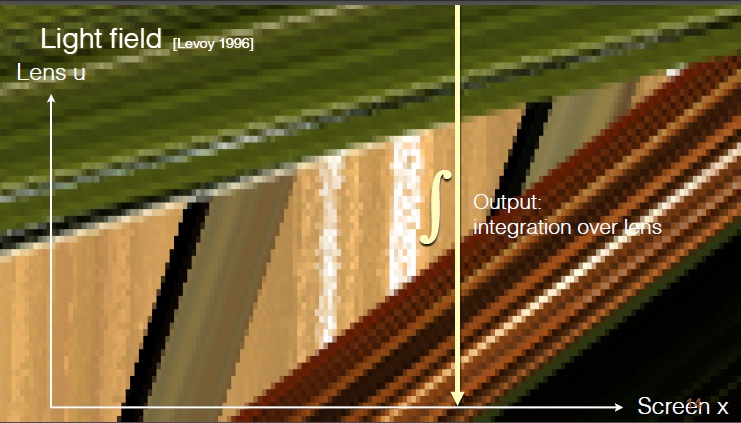
\includegraphics[scale=0.8]{./xu-plane.jpg}

  \small{Figure 1. Demonstration of the $xu$-plane in [1].}
\end{center}

The defocusing effect is depicted in Figure 1. For the simple pin-hole camera, for every $xy$-coordinate there exists exactly one $uv$-coordinate that contributes to the pixel, hence only one row in Figure 1 is effective for each $y$. However, for realistic cameras the out-of-focus points actually displace when viewed through different positions on the lens. This leads to the slant trajectories in Figure 1. For points on the focus, the trajectories are almost vertical.

\begin{center}
  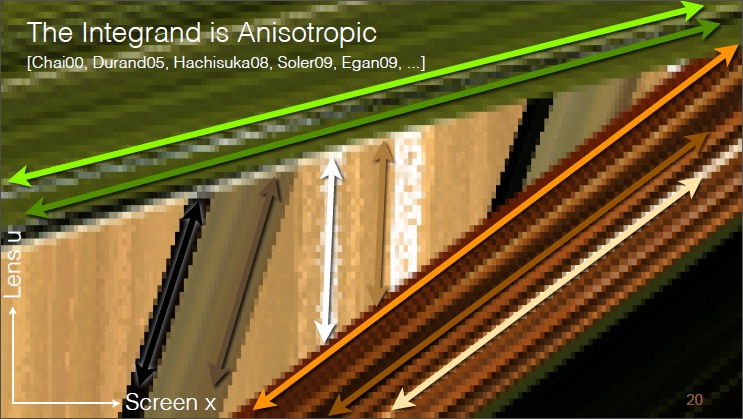
\includegraphics[scale=0.8]{./anisotropy.jpg}

  \small{Figure 2. The light field is anisotropic [1].}
\end{center}

On the other hand, the light field is actually anisotropic. Given a point in the scene, its contribution to the light field is approximately constant over different point on the lens as in Figure 2. The resulting image of the $xu$-plane hence consisting of several different lines segments, each resulting from some fixed point in the scene. This corresponds to the intuition that the scene should move smoothly when we stroll through the lens. The usual Monte-Carlo integration method (integrating over $u$) does not exploit this property but instead sampling the $xu$-plane vertically, thus obtaining signals with large variance at out-of-focus points.

\begin{center}
  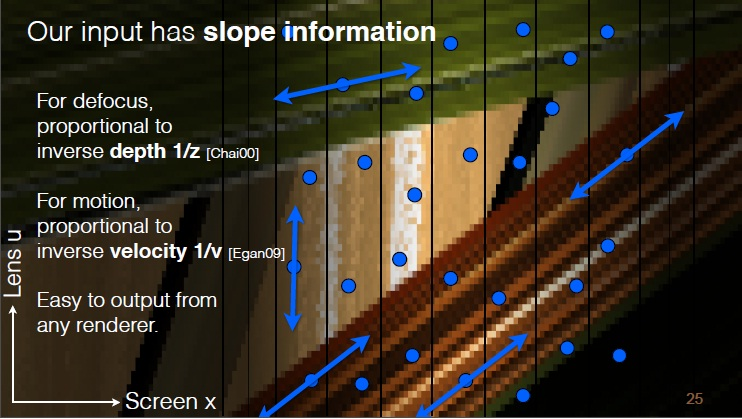
\includegraphics[scale=0.8]{./sample-slope.jpg}

  \small{Figure 3. (Sparse) samples with slopes [1].}
\end{center}

In the proposed system, the anisotropy of sampling points are utilized to reconstruct the light field. Given the relatively sparse input samples of the light field, the system estimates the slope of each sample by its depth with formula

\[ \frac{\partial u}{\partial x}\approx \frac{C_1}{z} + C_2 \]

where $C_1$, $C_2$ are predetermined constants drawn using the thin-lens approximation. Then for any reconstruction location $(\hat{x},\hat{y})$ on the image plane and any sample position on the lens $(\hat{u},\hat{v})$, the algorithm first moves each sample at $(x,y)$, $(u,v)$ along its trajectory to the new $(x',y')$, $(\hat{u},\hat{v})$ location (i.e. to the same horizontal line on the $xu$-, $yv$-plane). Visible samples $(x',y')$ near the point $(\hat{x},\hat{y})$ are then filter together to produce the radiance of the sample $(\hat{x},\hat{y})$, $(\hat{u},\hat{v})$.

The reconstruction technique is claimed to be applicable to a wider range other than defocus, such as motion blur and refocusing of the picture. I did not repeat those experiment, though.

\section{Algorithm and Implementation}
The algorithm works by first render a coarse version of the image, then re-render the image using dense, reconstructed samples on the light field. Given a reconstruction location $(\hat{x},\hat{y})$, $(\hat{u},\hat{v})$,

\begin{enumerate}
\item 
\end{enumerate}

\section{Experiment and Discussion}
\section{References}
\begin{enumerate}
\item Jaakko Lehtinen et al, \textit{Temporal Light Field Reconstruction for Rendering Distribution Effects}. Proceedings of ACM SIGGRAPH, 2011.
\item Pharr, M., and Humphreys, G. 2010. \textit{Physically Based Rendering, 2nd ed}. Morgan Kauffmann.
\item \textit{Scenes for PBRT}. \texttt{http://www.pbrt.org/scenes.php}
\end{enumerate}
\section*{Appendix A. Environment Setup and Compilation}
\end{document}